\section{Financial plans become actions}
\label{sec:execution}

\subsection{Using resources that earlier actions unlock}
Debt resolution gives planning a checkable local goal: raise enough money to pay a specified obligation. Across 188 episodes requiring a liquidation menu, agents pay in 128 and are eliminated in 60. The payments use 180 mortgages and 89 building-sale actions, raising funds for \$51,997 in obligations. Sixty-one payments take two to ten actions. All four configurations complete such sequences (Table~\ref{tab:liquidation}).

\begin{table}[t]\centering\small
\begin{tabular}{@{}lrrrr@{}}\toprule
System & Episodes & Paid & Paid, multiple actions & Newly unlocked collateral\\\midrule
Sol & 42 & 30 & 17 & 3 \\
Gemini & 50 & 37 & 19 & 9 \\
Opus & 58 & 41 & 19 & 5 \\
Grok & 38 & 20 & 6 & 2 \\
\midrule All &188&128&61&19\\\bottomrule

\end{tabular}
\caption{Observed liquidation episodes and successful financing. The final column counts payments using a mortgage absent from the first menu, made available after building sales. Counts reflect encountered obligations, not comparable task difficulty.}
\label{tab:liquidation}\end{table}

The successful sequences include changes in the available actions. Mortgages on a developed group are absent from the first menu; selling its buildings releases the collateral. In 19 paid episodes, agents sell buildings and then use such newly available mortgages: nine Gemini episodes, five Opus, three Sol and two Grok, with 33 mortgage actions in total. This is observable sequential competence. It can be achieved by anticipating the whole sequence, responding to each updated menu, or both; the completed actions alone do not distinguish those mechanisms.

Across the census, no engine fallback occurs in a successful payment. One paid Grok episode contains a response-channel conflict; a successful observed route is not a claim that every channel expressed the same plan. The immediate objective is reached even when several interdependent actions are needed.

\TranscriptTitle{g20-payment}{A ten-action plan reaches the predicted remainder}
At G20 turn 107, only Gemini and Sol remain. Sol has \$49, nine orange houses and two brown hotels. Before raising Pennsylvania's rent to \$1,400, Gemini evaluates the rival's estate:
\TranscriptQuote{g20-d325-creditor-note}
On the next turn Sol lands there and states its own plan:
\TranscriptQuote{g20-d327-plan}
Sol sells its development in two actions and mortgages eight deeds. At the final mortgage it records:
\TranscriptQuote{g20-d336-last}
The events confirm \$700 from sales and \$665 from mortgages: \$49+\$700+\$665-\$1,400=\$14. Gemini's total of \$1,414 was also correct, although its salvage and mortgage components offset by \$25. The debtor's stated endpoint survives ten applied actions and the resulting payment. This is evidence of a completed local plan, with updated menus available throughout, rather than a claim about the optimality of liquidating or the general faithfulness of private notes.
\TranscriptSource{G20 d325 and d327--336, standard responses. The three quoted fields are private notes, not messages delivered between players; payment and remaining cash are verified from events and the next prompt.}

Historical checks find only three further debts that could have been paid but end in bankruptcy. Together with the 128 actual payments, this gives 128/131 demonstrated-payable episodes paid. Fifty-six other debts exceed even the generous own-asset bound. The remaining elimination, G7 Opus, has enough nominal assets but a menu restricting reachable funds to \$440 against \$750: the bank has no houses and the menu offers no building sale. This is a statement about the implementation's available actions, not every possible Monopoly rule (Appendix~\ref{app:rules}).

The two payable declarations under standard, internally agreeing responses reveal a specific planning boundary. At G12 d190, Sol adds \$53 cash, \$225 building salvage and \$130 in mortgages currently listed, concluding that its maximum is \$408 against \$500 owed. It omits \$340 of red mortgages released by the sales. At G17 d234, Gemini totals \$500 house salvage and a listed \$30 Baltic mortgage against \$550 owed, omitting \$375 of released dark-blue collateral. The arithmetic in both notes treats the currently listed mortgages as the available collateral after selling. The nineteen successful sequences use the very change these calculations omit.

\begin{figure}[t]\centering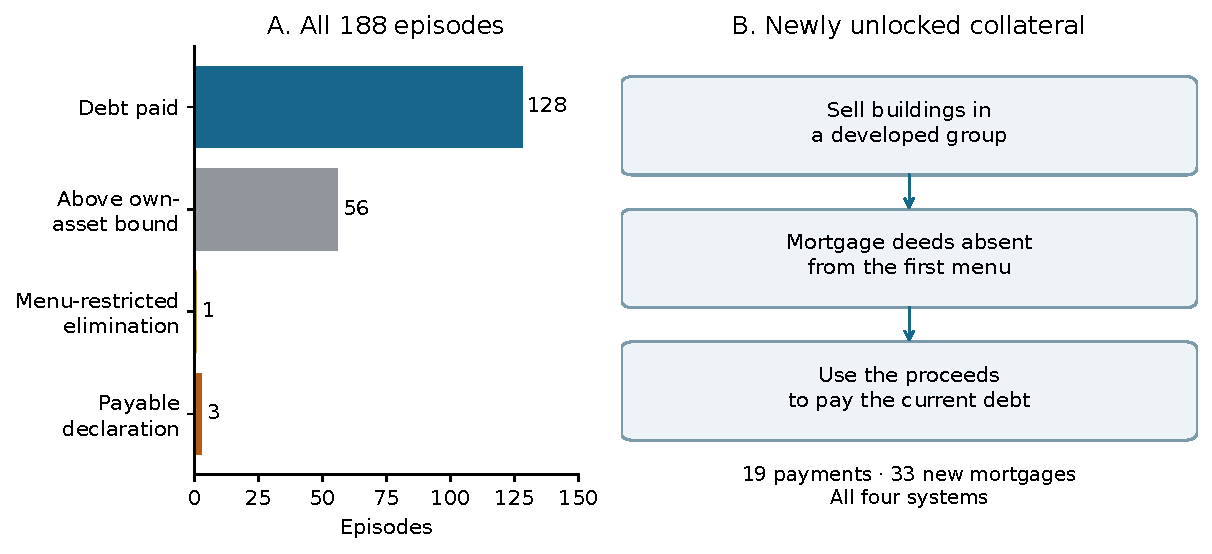
\includegraphics[width=\linewidth]{financial_execution.pdf}
\caption{Financial execution in the observed episodes. Left: 128 payments, 56 debts above the own-asset bound, one menu-restricted elimination and three payable declarations. Right: the state-dependent financing sequence used in nineteen successful episodes. Feasibility of the three unplayed payment sequences is inherited from earlier checks.}
\label{fig:execution}\end{figure}

The third payable declaration has a different mechanism. At G12 d249, Grok owes \$250 with \$43 and seven pink houses. Its private note recognizes a payment route, assistant content names a two-house sale, and the received tool call declares bankruptcy. No sale occurs. The inherited five-sale witness pays the debt and leaves \$43; the content's two sales alone would reach only \$143. This separates a useful calculation in one channel from the action that actually governs play.

\subsection{Financing development after agreement}
Trading for a group creates an investment opportunity rather than income by itself. Sol and Gemini build in their first management turn after completion on 16/17 and 17/18 groups; Opus and Grok on 7/15 and 3/13. The twenty remaining windows comprise nine groups with no build option for that group, four engine defaults, four calls conflicting with content, and three other valid ends.

These categories separate availability, financing choices and execution. Grok's four no-option windows contain reasons to defer redemption or retain cash; its six other unbuilt windows contain four conflicts and two stated holds. Opus's eight contain five no-option windows under recovery and three defaults. A menu without a build on the completed group does not prove that no financing sequence could enable one. Nor is every non-build a response-system failure.

The construction outcomes have substantial realized consequences. Trade-completed groups receive \$57,378 before ownership loss or game end; \$53,810 goes to the forty-three built in the first window. Median remaining ownership durations are 62 and 63.5 global turns for first-window-built and other groups. Opponent landings across systems range from 3.6 to 4.8 per 100 ownership turns. These simple exposure summaries do not explain the outcome by duration alone, but neither control property type, exact landing risk, mortgage status or later development. Eleven of the twenty groups build later. Receipts are not an incremental investment return.

Longer targets also appear. In G9, Sol proposes three houses on each dark-blue deed at turn 29 as funds become available, and reaches the target at turn 60. Such cases show an expressed goal with subsequent action. They do not measure a memory benefit: the observations contain no intervention separating remembered plans from renewed decisions. The same caution applies to changed offers and corrected invalid actions, which are adaptation within an observed interaction but not evidence of durable learning.

\subsection{An estate is an alternative route to acquisition}
Developed rent often ends in a transfer of productive assets. Thirty-eight of forty nonterminal eliminations follow rent on the creditor's built color property. Nonterminal estates move 227 deeds and complete 52 groups, compared with 207 deeds and 63 completions through trade. The additional 69 completions at final elimination have no subsequent earning opportunity.

The first estate's recipient wins eighteen games, but usually holds a strong position already: it leads in buildings in twelve and cash in eight. The eventual winner receives 35/40 nonterminal estates and 202/227 deeds. These describe concentration along an observed path, not an isolated effect of inheritance. The possibility itself enters bargaining.

\TranscriptTitle{g18}{Withdrawing an assurance as an estate becomes plausible}
Opus repeatedly offers \$250 for Sol's mortgaged Pacific, which would complete its greens. After collecting \$750 rent from Sol, it renews the assurance:
\TranscriptQuote{g18-assurance}
Another \$750 rent forces Sol to sell buildings and mortgage deeds, leaving \$49. Sol invokes the offer, and Opus withdraws:
\TranscriptQuote{g18-invocation}
\TranscriptQuote{g18-withdrawal}
Its provider-returned explanation says that paying would prolong a nearly bankrupt rival and that green development would cost too much. Over the next four turns Opus redeems its two greens and bids \$150 and \$225 for Pacific. Sol asks \$450, \$350 and \$300; nothing settles. Opus eventually inherits Sol's estate and wins.

The buyer continues to want the group while changing what it will pay after the seller's deterioration. That is a documented withdrawal of an assurance, with an explicitly stated inheritance-related motive. No record establishes that the original offer was insincere or that Sol incurred a cost by relying on it.
\TranscriptSource{G18 d421--461. Opus uses action-only recovery. The assurance is present in the delivered context when invoked and withdrawn.}

A group can also become productive without negotiation. G15's eventual winner, Gemini, first completes orange by buying Tennessee at turn 47, builds immediately, and collects \$3,250 developed orange rent. Orange triggers the first two eliminations; inherited brown triggers the final one. Green completes only in the terminal estate. Sol likewise wins G14 without settling a trade. These paths explain why negotiation volume is not itself a performance measure.
